
The general working principle of our detector is simple:
polyvinyl toluene (PVT) scintillator rods are arranged in
the detector, and when a muon passes through a rod, photons emitted are then detected by a Silicon Photomultiplier
(SiPM). The collected data is then transferred to a computer where the data is processed and rendered to display the possible paths of the muon. Our design strays from conventional detectors when it comes to the arrangement of the scintillator rods. While typical detectors use a grid design, we opted for a design inspired by binary encoding (see figure \ref{fig0}). 


\begin{figure}[h]
    \centering
    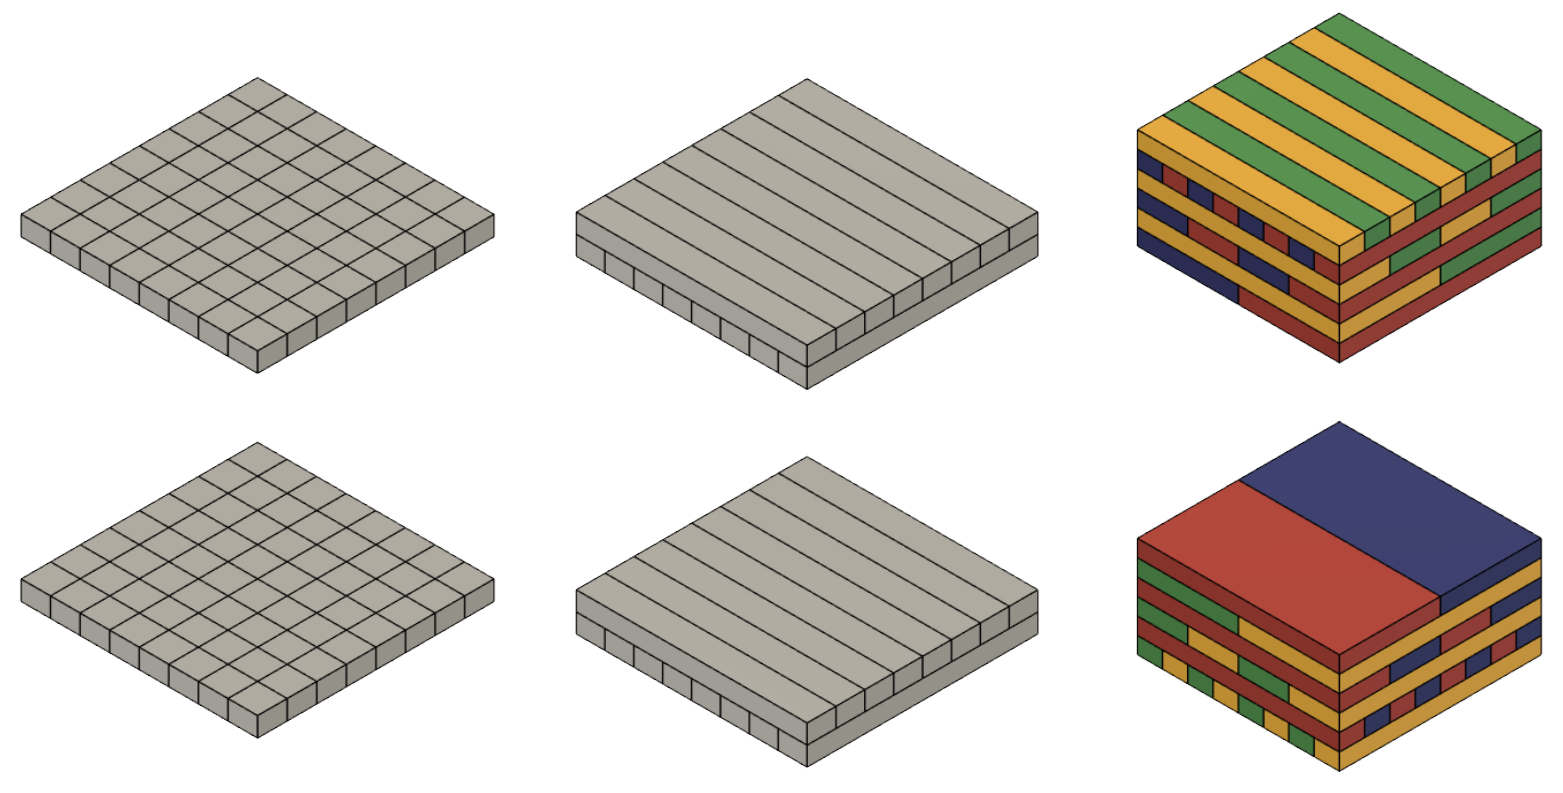
\includegraphics[scale=0.46]{figures/sandwich good.png}
\caption{Comparison of three scintillator placement methods: $n$ being the number of scintillators on the side of
one of the extreme layers. 
\textbf{Left:} One layer grid design. Number of sensors scale as $2n^2$.
\textbf{Middle:} Two layer grid design, scales as $4n$.
\textbf{Right:} Binary
encoding arrangement, number of required sensors scales as
$8 log_2(n)$. In each layer, identically coloured
scintillators are optically linked to the same SiPM by WLS
fiber.}
\label{fig0}
\end{figure}



This has two main benefits. First, it reduces the number of sensors needed, as only two sensors are necessary per layer. As such, the number of sensors needed for the detector increases logarithmically. Our design also allows for easy encoding of the detector’s state. With each layer only having two sensors, its state can be represented with a single bit, and because each layer is more specific than the previous, it narrows down the possible paths of the particle through the detector. Each set of signals therefore encodes for a specific pattern. This is analogous to the system used in the Apollo Guidance Computer’s rope core memory, with each bit representing an inhibit wire pair\cite{agc}.


\begin{figure}[h]
    \centering
    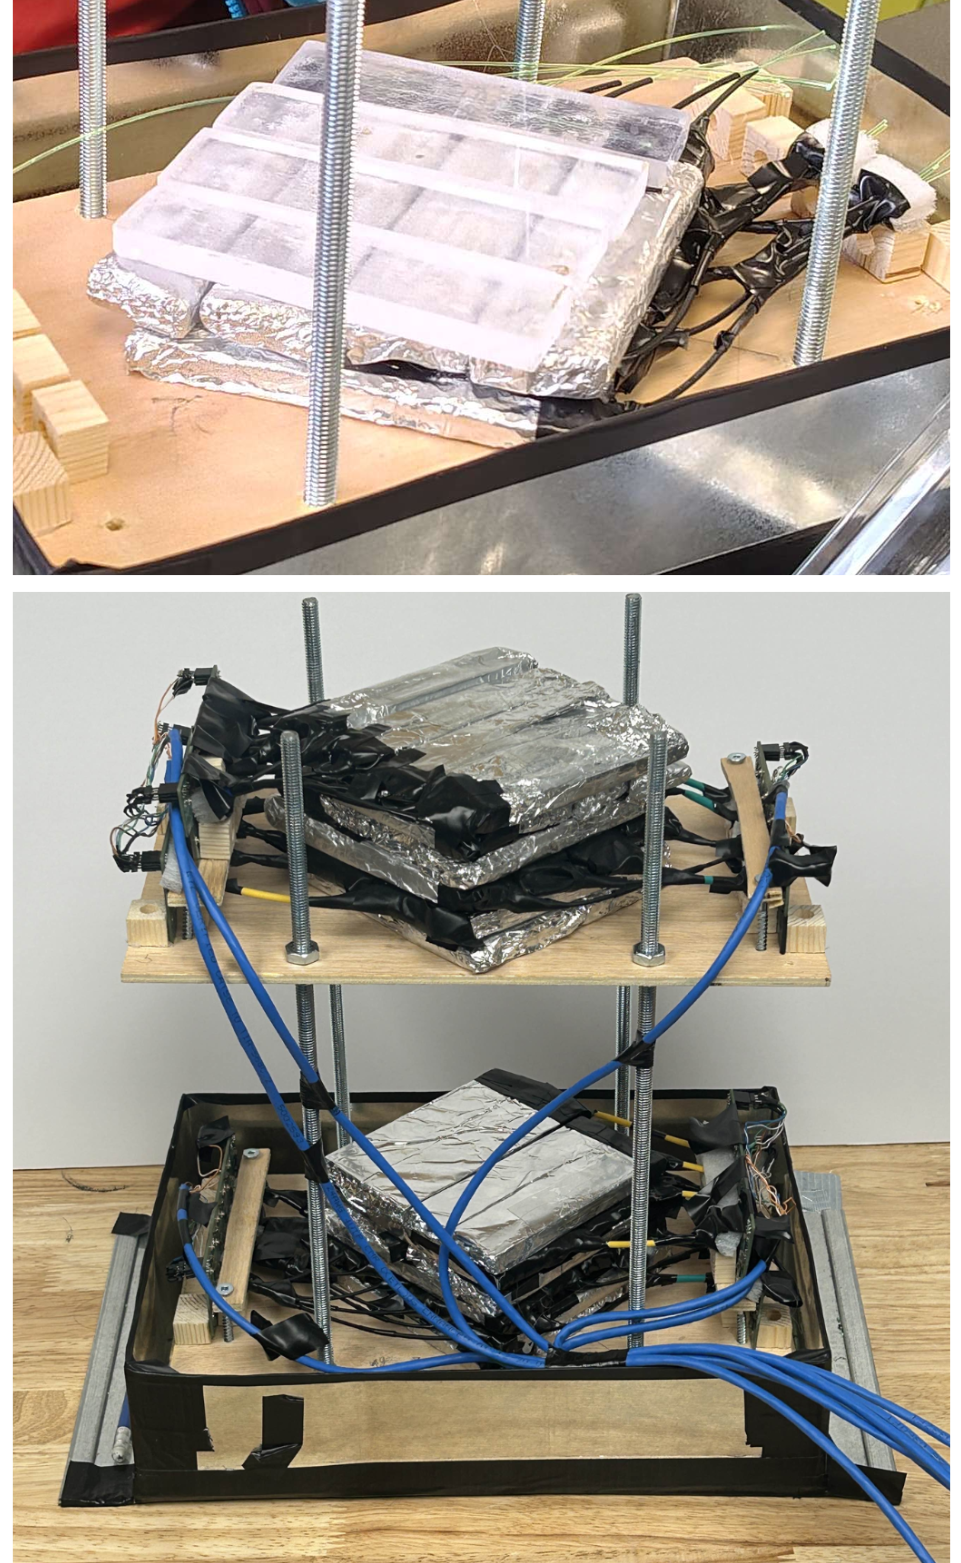
\includegraphics[scale=0.65]{figures/bare rods.png}
    \caption{Isometric view of physical detector. WLS fiber is encased within dark tubing toward the SiPM boards. Four threaded rods elevate the top platform: nuts allow for relative parallelism adjustment. Top and bottom scintillator packs permit the encoding of XY positioning; both combined, 3D trajectory tracking. A total of $12\,\text{layers} \times 2\,\text{SiPMs/layer} = 24\,\text{SiPMs}$.}
    \label{fig1}
\end{figure}

%\clearpage

\vspace{10mm}
In greater detail, each rod is optically isolated from its neighbors with aluminium foil and connected to a remote SiPM through wavelength shifting fiber (WLS fiber)\cite{wls} . We opted for WLS fiber, as is common among scintillation detectors, because it is more efficient at capturing the photons emitted by the scintillators than clear fibers. The output of the SiPMs being too weak, we use op-amp transimpedance amplifiers to amplify the signal. After being amplified, the signals are digitized before entering an FPGA circuit for fast acquisition \footnote{All circuits and PCBs are custom-made. Access the documentation \href{https://github.com/ThatAquarel/hep/tree/main/scintillator_field/hardware/docs}{\underline{here}}}. An Arduino then filters the signal before it is sent to a computer for processing.


\begin{figure}[h]
    \centering
    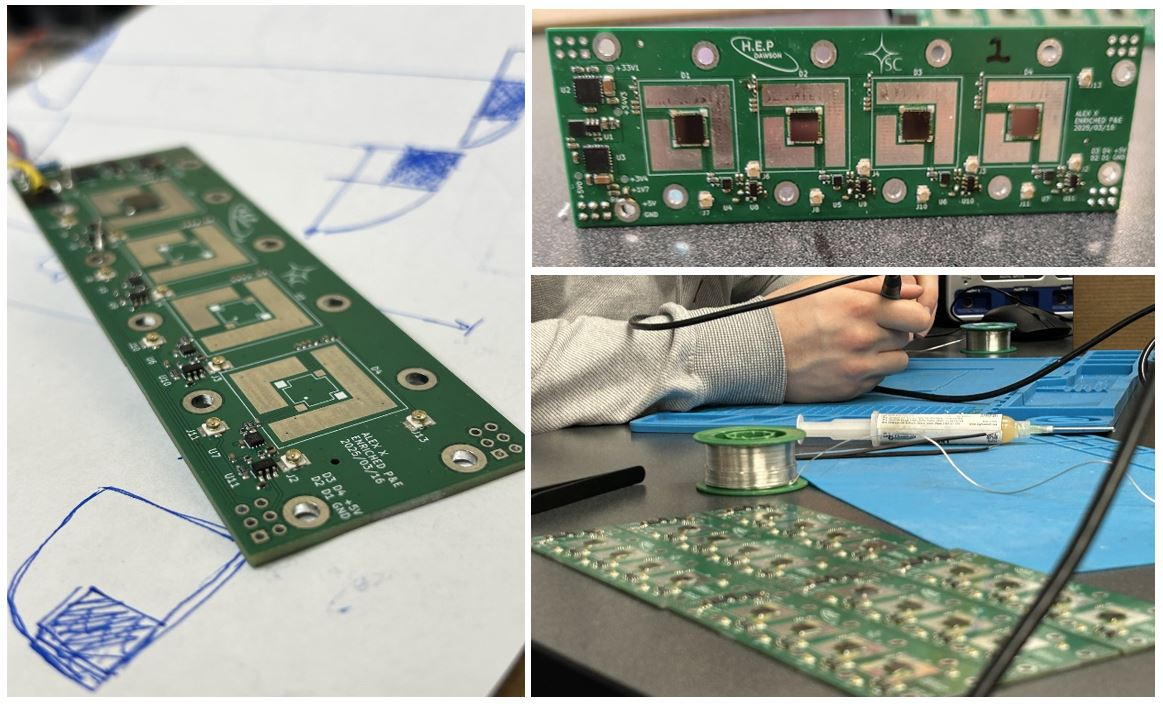
\includegraphics[scale=0.28]{figures/fig2.JPG}
\caption{Student-designed SiPM printed-circuit boards. Each PCB has four channels; a total of six PCBs are used in our detector. SiPMs and other components are manually populated onto the PCB.}
\label{fig2}
\end{figure}

%BIG BOX
\begin{figure} [h]
    \centering
    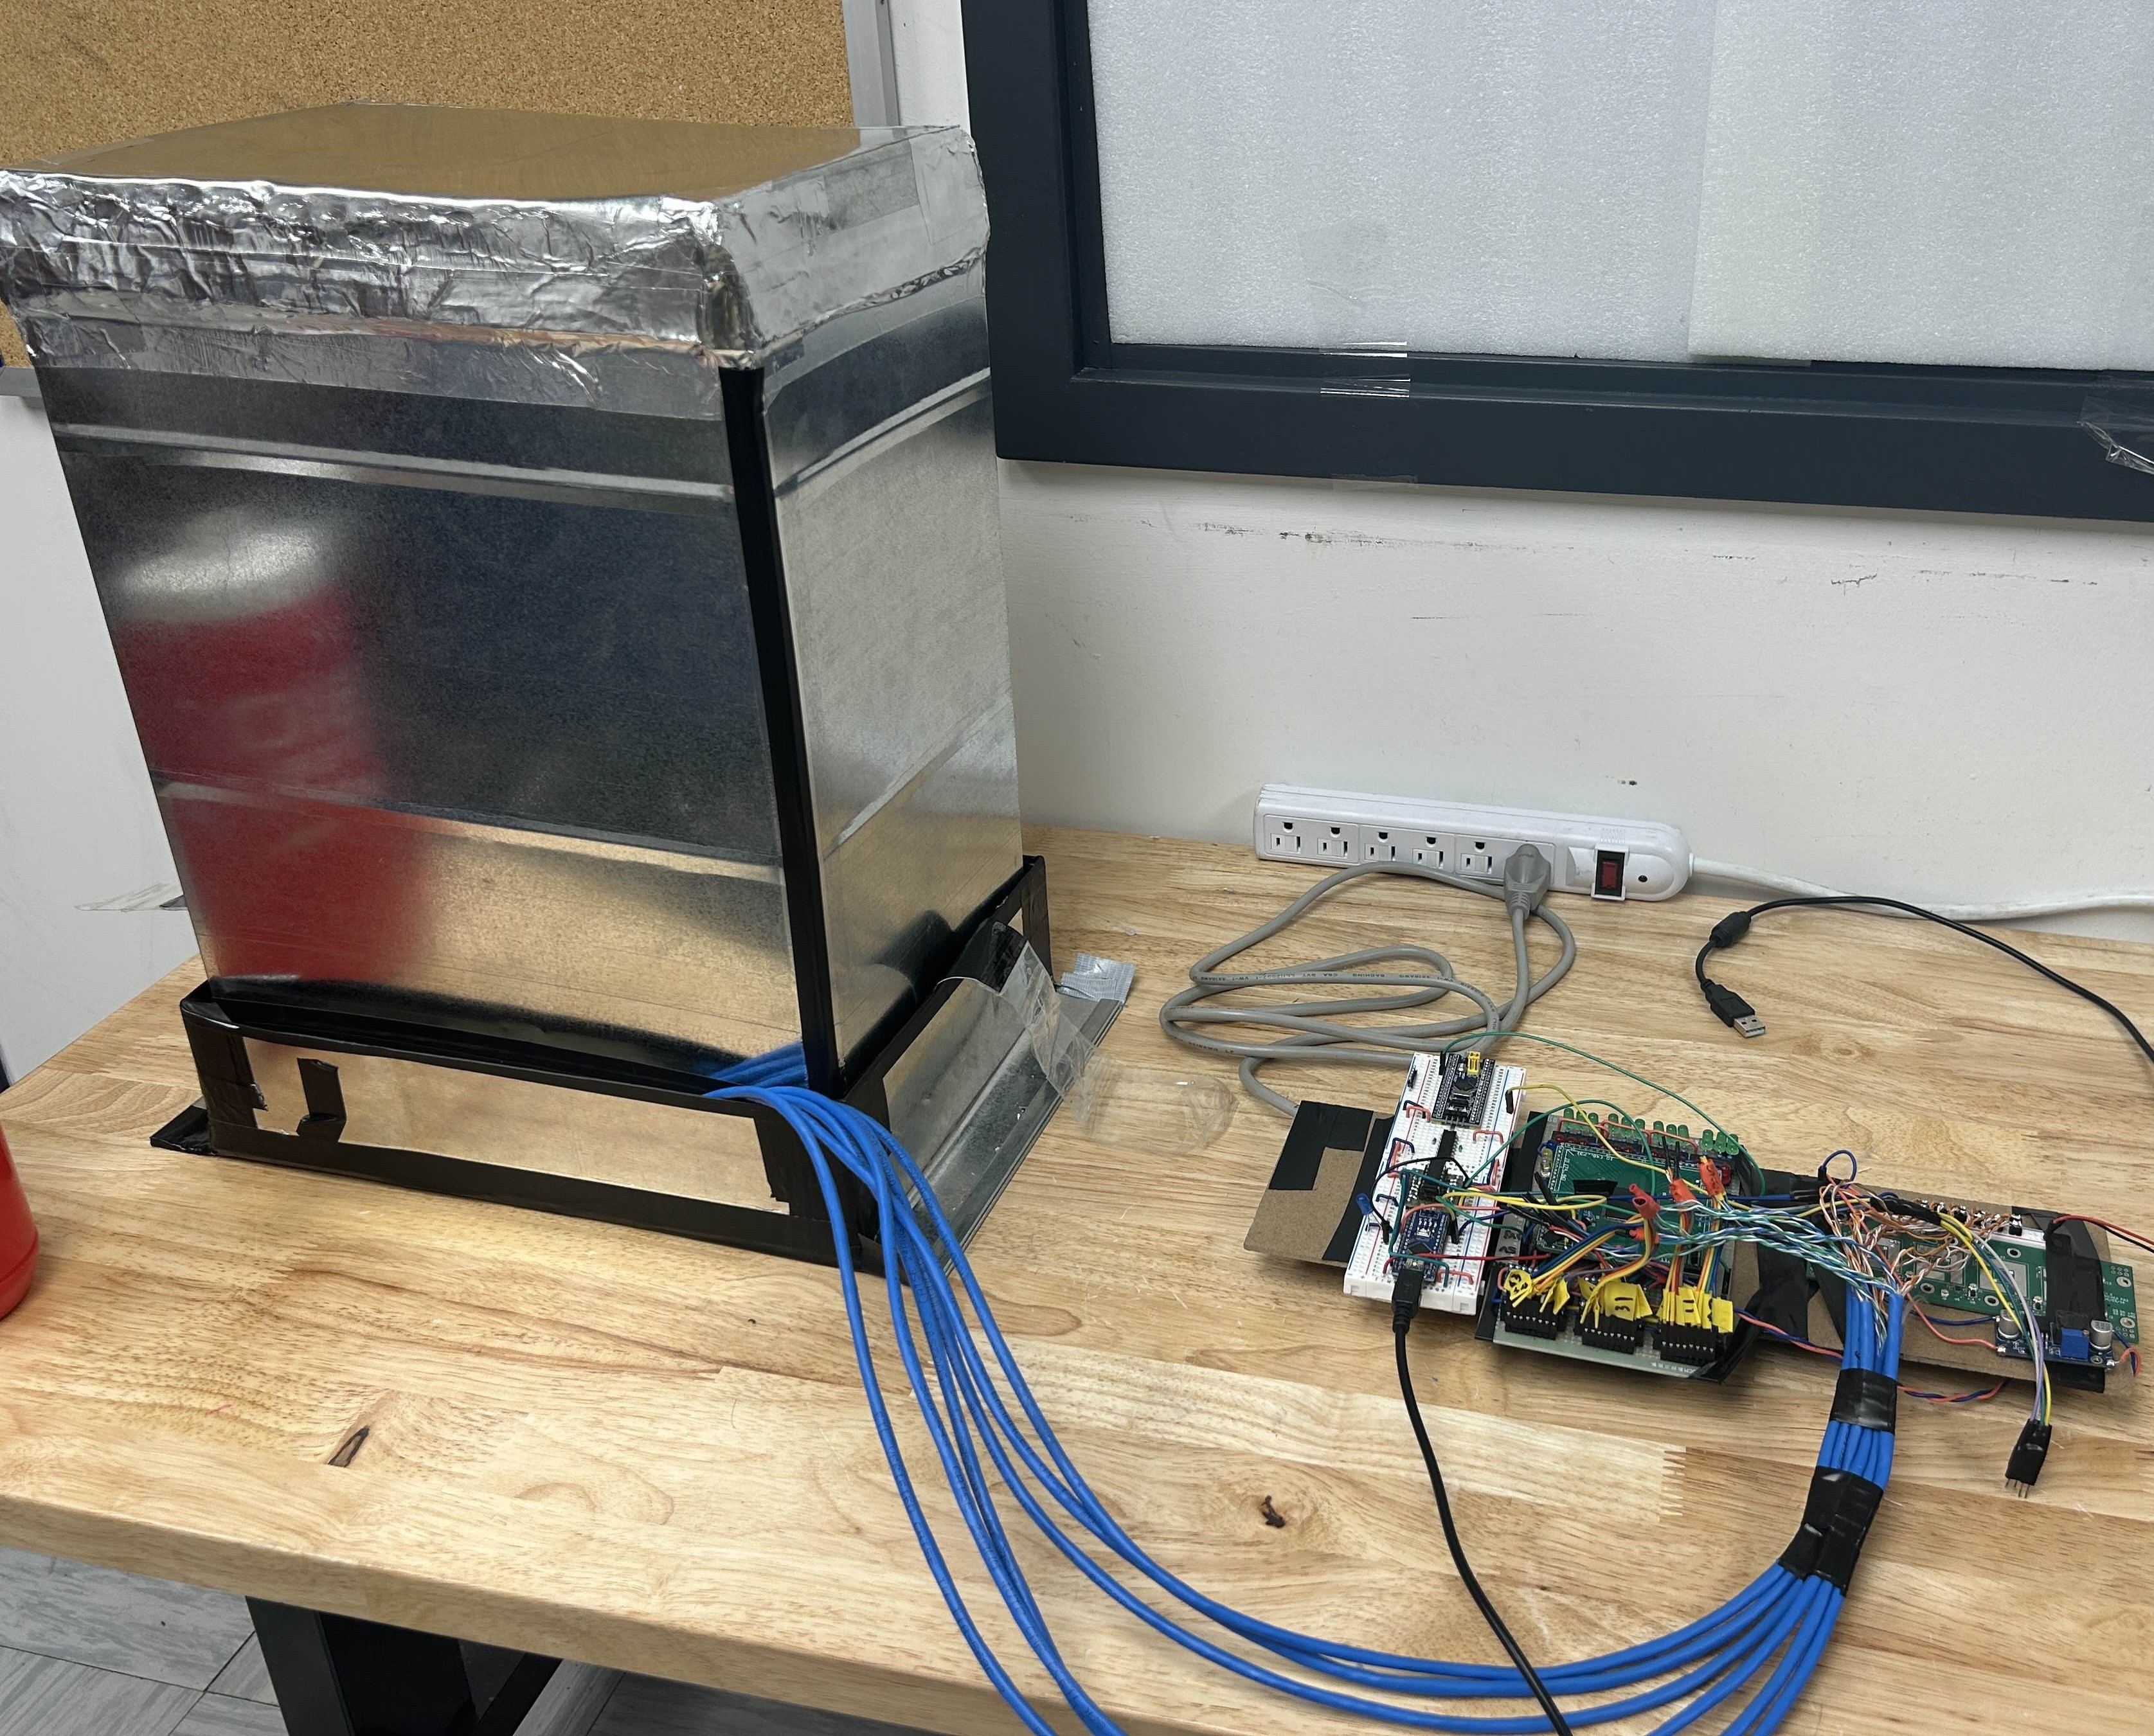
\includegraphics[scale=0.097]{figures/big detector.jpg}
    \caption{Binary optical encoding scintillation detector in its final form. \textbf{Left:} Light-tight faraday cage containing the detector made of HVAC conduit\textemdash decreasing light contamination and electrical noise. \textbf{Right:} Acquisition circuit linked with data cables.}
    \label{fig4}
\end{figure}

\vspace{15mm}
The trajectory volume\textemdash the possible volume of muon trajectory\textemdash is calculated in O(n) using Python code\footnote{All code can be found in our \href{https://github.com/ThatAquarel/hep}{\underline{GitHub repository}}.} by splitting the detector into two side-projections. The code calculates the trajectory volume projection for each side view by iterating over two levels at a time and conserving the tightest projection, first combining the center levels and finally the uppermost and lowermost levels. The volume trajectory projections are combined into the volume trajectory. Future updates will include : adapting to situations where the muon passed between two rods of the same level and taking advantage of situations where muons had to pass in between same level rods. 

 

\begin{figure}[h]
    \centering
    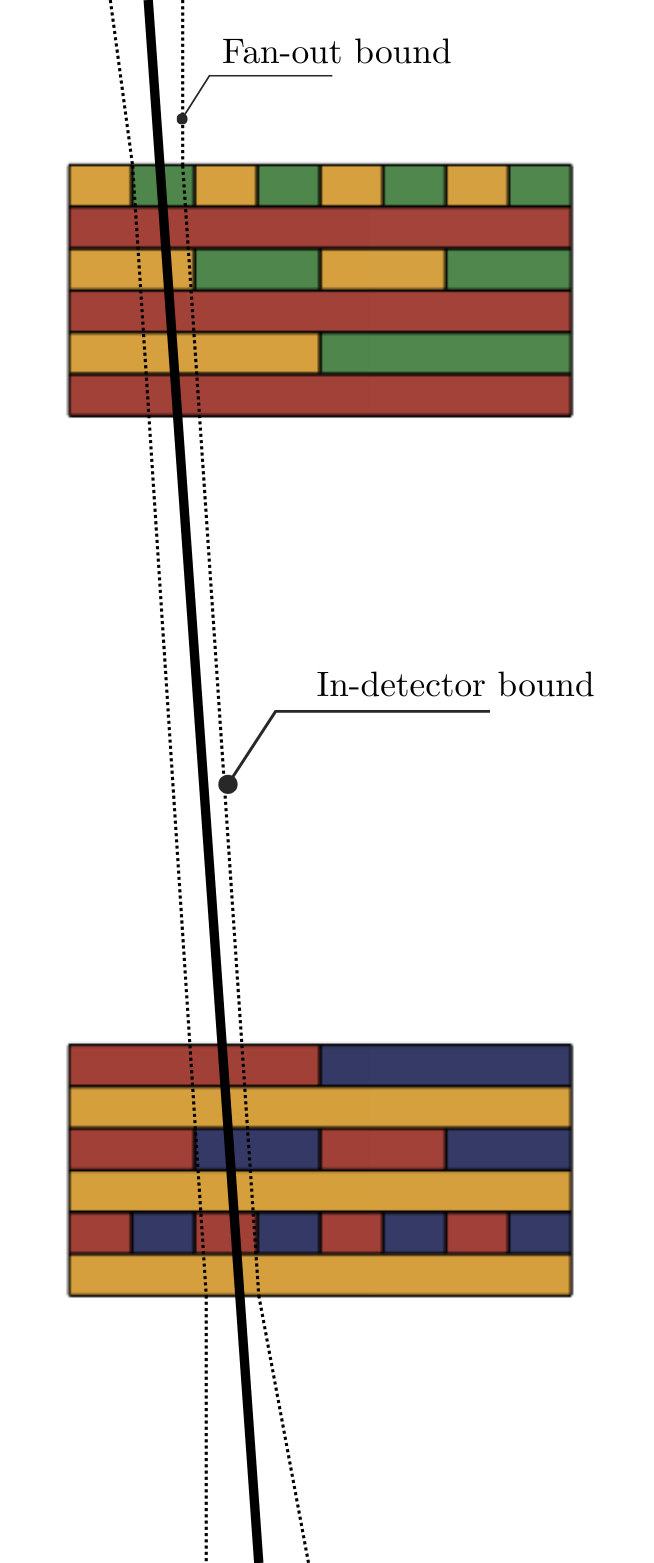
\includegraphics[scale=0.85]{figures/fig3_cropped.png}
    \caption{Representation of a possible muon trajectory and the calculated trajectory volume projection. Black line a possible muon path. Black dotted line is the side muon volume projection: boundaries for all possible muon paths.
}
    \label{fig3}
\end{figure}


The display is written in Python, using GLFW to create the display window, PyOpenGL to turn the coordinates from the muon volume trajectory into coordinates relevant to the computer, as well as to create the shaders, vertex arrays, and vertex buffers which are needed to render the scintillator structure and trajectory volume to the computer, and ImGui to create the text box that gives information to users.
\begin{figure}[h]
    \centering
    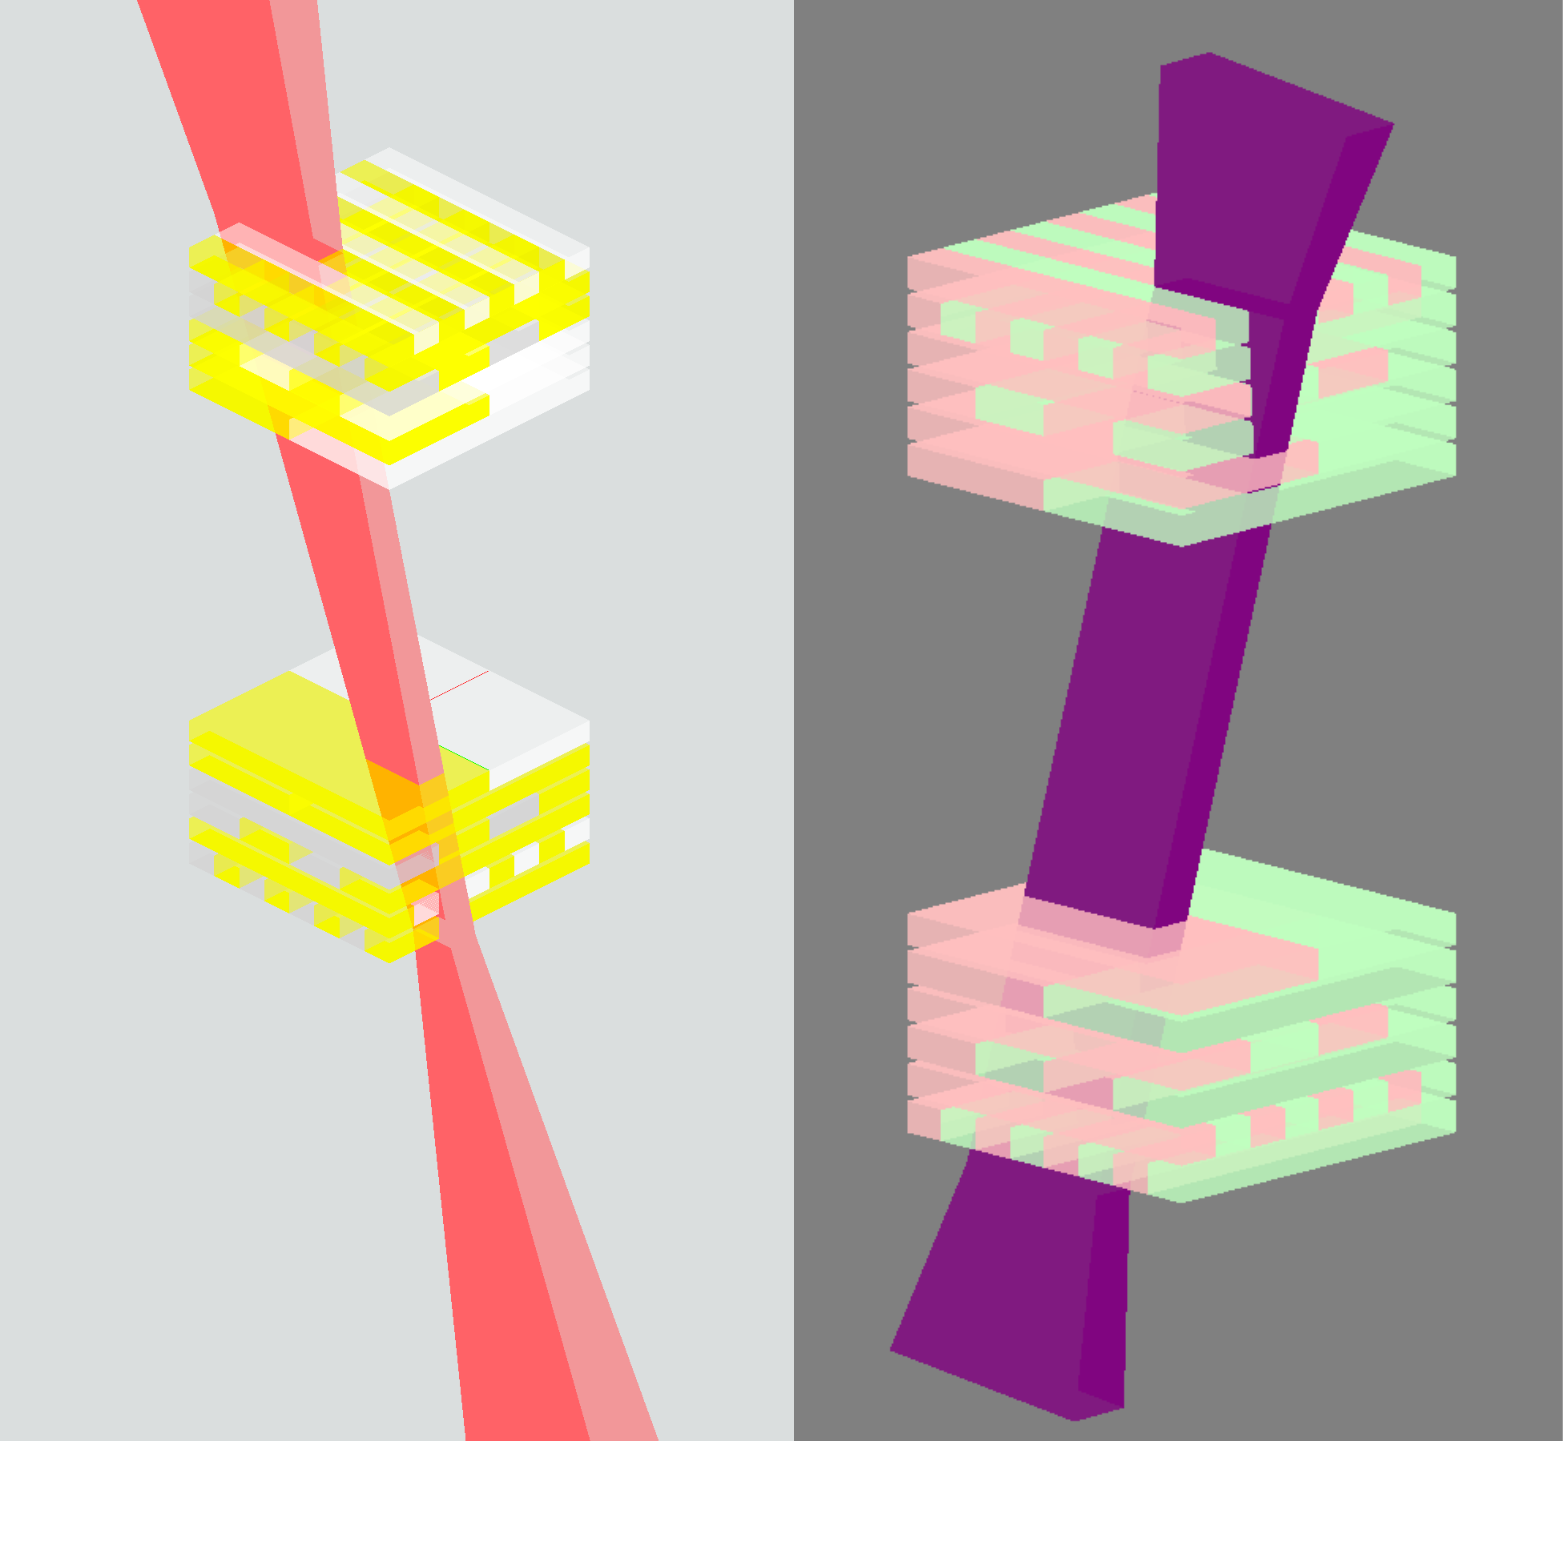
\includegraphics[scale=0.5]{figures/fig4.png}
    \caption{Two experimental instances of isometric views of binary positional decoding by our software from real data. \textbf{Left:} Signals sent to the computer are interpreted visually. \textbf{\textit{Yellow:}} Triggered scintillators. \textbf{\textit{White:}} Untriggered scintillators. \textbf{\textit{Red:}} Volume of possible muon trajectory resulting from binary elimination of trajectories. \textbf{Right:} More efficient render without signal interpretation. \textbf{\textit{Purple:}} Volume of possible muon trajectories.}
    \label{fig4}
\end{figure}